\documentclass[12pt]{article}
\usepackage[english]{babel}
\usepackage[utf8x]{inputenc}
\usepackage{amsmath}
\usepackage{tikz}
\usetikzlibrary{arrows,automata}
\begin{document}
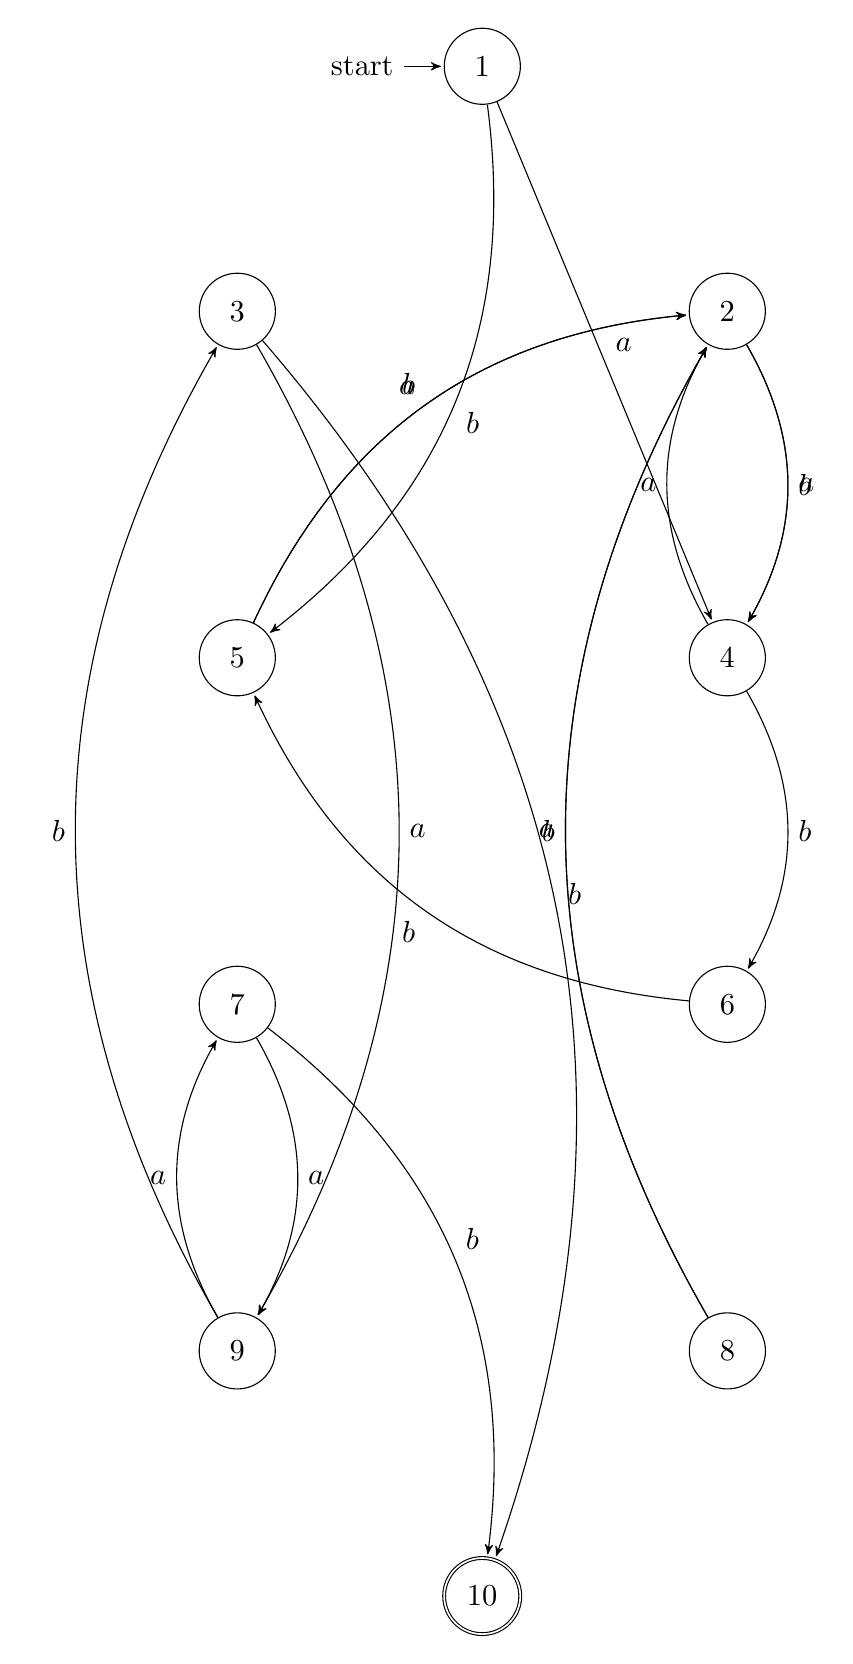
\begin{tikzpicture}[->,>=stealth',shorten >=1pt,auto,node distance=4cm, scale = 1.1,transform shape]
\node[state,initial] (0)   {$1$};
\node[state]  (1) [below right of = 0] {$2$};
\node[state]  (2) [below left of = 0] {$3$};
\node[state]  (3) [below of = 1] {$4$};
\node[state]  (4) [below of = 2] {$5$};
\node[state]  (5) [below of = 3] {$6$};
\node[state]  (6) [below of = 4] {$7$};
\node[state]  (7) [below of = 5] {$8$};
\node[state]  (8) [below of = 6] {$9$};
\node[state,accepting] (9) [below right of = 8] {$10$};
\path (0) edge node {$a$}(3)
   (0) edge [bend left] node {$b$}(4)
   (1) edge [bend left] node {$a$}(3)
   (1) edge [bend left] node {$b$}(3)
   (2) edge [bend left] node {$a$}(8)
   (2) edge [bend left] node {$b$}(9)
   (3) edge [bend left] node {$a$}(1)
   (3) edge [bend left] node {$b$}(5)
   (4) edge [bend left] node {$a$}(1)
   (4) edge [bend left] node {$b$}(1)
   (5) edge [bend left] node {$b$}(4)
   (6) edge [bend left] node {$a$}(8)
   (6) edge [bend left] node {$b$}(9)
   (7) edge [bend left] node {$a$}(1)
   (7) edge [bend left] node {$b$}(1)
   (8) edge [bend left] node {$a$}(6)
   (8) edge [bend left] node {$b$}(2)
;
\end{tikzpicture}
\end{document}
